\documentclass[12pt,titlepage]{article}
\usepackage[utf8]{inputenc}
\usepackage[indonesian]{babel}
\usepackage{geometry}
\geometry{a4paper, margin=2.5cm}
\usepackage{graphicx}
\usepackage{amsmath}
\usepackage{amsfonts}
\usepackage{booktabs}
\usepackage{listings}
\usepackage{xcolor}
\usepackage{hyperref}

\definecolor{codegreen}{rgb}{0,0.6,0}
\definecolor{codegray}{rgb}{0.5,0.5,0.5}
\definecolor{codepurple}{rgb}{0.58,0,0.82}
\definecolor{backcolor}{rgb}{0.95,0.95,0.92}

\lstset{
    backgroundcolor=\color{backcolor},
    commentstyle=\color{codegreen},
    keywordstyle=\color{magenta},
    numberstyle=\tiny\color{codegray},
    stringstyle=\color{codepurple},
    basicstyle=\ttfamily\footnotesize,
    breakatwhitespace=false,
    breaklines=true,
    captionpos=b,
    keepspaces=true,
    numbers=left,
    numbersep=5pt,
    showspaces=false,
    showstringspaces=false,
    showtabs=false,
    tabsize=2
}

\begin{document}

\section*{Judul Tugas}
\textbf{Tugas Autoencoder}: Training di Kaggle dan Rekonstruksi Citra Fashion-MNIST melalui Decoder

\section*{Nama dan NIM}
\begin{itemize}
	\item \textbf{Nama Mahasiswa:} M. Faridh Maulana
	\item \textbf{NIM:} 452024611065
	\item \textbf{Program Studi:} Teknik Informatika, Universitas Darussalam Gontor
\end{itemize}

\section{Penjelasan Singkat Arsitektur Autoencoder dan VAE}
Autoencoder konvensional bekerja dengan memetakan input berdimensi tinggi ke dalam representasi vektor tunggal diskrit di dalam \textit{bottleneck layer} (Encoder), lalu merekonstruksinya kembali (Decoder). Namun, pendekatan ini membuat \textit{latent space} bersifat diskontinu sehingga sulit digunakan untuk pemodelan generatif.

Sebagai solusinya, digunakan \textbf{Variational Autoencoder (VAE)}. Berbeda dengan Autoencoder biasa, VAE memetakan input ke dalam bentuk distribusi probabilitas kontinu yang didefinisikan oleh parameter rata-rata ($\mu$) dan log-varians ($\log \sigma^2$). Guna memungkinkan proses \textit{backpropagation} berjalan menembus sampling stochastic tersebut, diterapkan \textit{Reparameterization Trick}:
\begin{equation}
	z = \mu + \sigma \cdot \epsilon, \quad \text{dimana } \epsilon \sim \mathcal{N}(0, I)
\end{equation}

Arsitektur model yang diimplementasikan terdiri atas:
\begin{enumerate}
	\item \textbf{EncoderVAE:} 3 Layer \textit{Convolutional 2D} dengan \textit{stride=2} untuk mereduksi dimensi spasial citra input ($1 \times 32 \times 32 \rightarrow 32 \times 16 \times 16 \rightarrow 64 \times 8 \times 8 \rightarrow 128 \times 4 \times 4$), diikuti dengan proses \textit{flattening} dan pemetaan linear menuju pasangan vektor $\mu$ dan $\log \sigma^2$ sesuai ukuran \textit{latent dimension}.
	\item \textbf{Decoder:} Menerima sampel vektor dari \textit{latent space}, memetakan kembali ke dimensi fitur awal melalui layer linear ($2048$), melakukan \textit{unflattening} menjadi matriks fitur, dilanjutkan dengan 3 layer \textit{ConvTranspose2d} serta diakhiri fungsi aktivasi \textit{Sigmoid} untuk memproyeksikan piksel ke rentang $[0, 1]$.
\end{enumerate}

\section{Penjelasan Proses Training di Kaggle}
Proses \textit{training} model dilakukan menggunakan \textbf{environment runtime} berbasis komputasi awan di platform Kaggle. Spesifikasi parameter dan tahapan eksekusi diatur sebagai berikut:
\begin{itemize}
	\item \textbf{Dataset:} Menggunakan Fashion-MNIST yang terdiri atas gambar pakaian berukuran asli $28 \times 28$. Pada proses \textit{data pipeline}, citra di-resize menjadi $32 \times 32$ piksel dan dikonversi ke dalam representasi Tensor.
	\item \textbf{Hiperparameter:} \textit{Learning rate} diatur pada nilai $10^{-3}$, ukuran \textit{batch size} ditetapkan sebesar $128$, dengan total masa latih sebanyak $10$ epoch per eksperimen dimensi laten.
	\item \textbf{Fungsi Optimizer:} Menggunakan algoritma \textit{Adam Optimizer} untuk pembaruan bobot jaringan secara adaptif.
	\item \textbf{Akselerasi Perangkat Keras:} Kompilasi grafis didukung penuh oleh pemanfaatan kartu grafis (GPU) eksternal NVIDIA yang tersedia pada komputasi lingkungan Kaggle demi mempercepat kalkulasi matriks \textbf{forward} dan \textbf{backward pass}.
\end{itemize}

\section{Hasil Grafik Loss}
Pada pengamatan hasil log logaritma \textbf{training}, ditemukan nilai nominal loss fungsional yang berada pada rentang puluhan ribu (sekitar $50.285$ turun hingga $44.347$ pada dimensi 2). Hal ini dikonfirmasi \textbf{benar dan valid} secara matematis.

Fenomena ini terjadi karena pada perancangan fungsi \textit{VAE Loss}, komponen \textit{Reconstruction Loss} dihitung menggunakan metode \textit{Binary Cross Entropy} (BCE) dengan parameter \lstinline|reduction='sum'|. Jaringan melakukan akumulasi total \textit{error} piksel dari keseluruhan data di dalam satu \textbf{batch}. Dengan formulasi matematis:
\begin{equation}
	\text{Total Elemen Piksel per Batch} = 128 \text{ (Batch Size)} \times 1024 \text{ (Total Pixel Image)} = 131.072
\end{equation}
Apabila nilai total loss tersebut dibagi secara rata oleh total elemen piksel per batch, maka didapatkan nilai \textit{BCE Loss} murni sebesar $\approx 0,33$ per piksel, sebuah parameter nilai loss yang sangat ideal untuk model generatif yang sedang mengalami konvergensi secara optimal.

\begin{figure}[htbp]
	\centering
	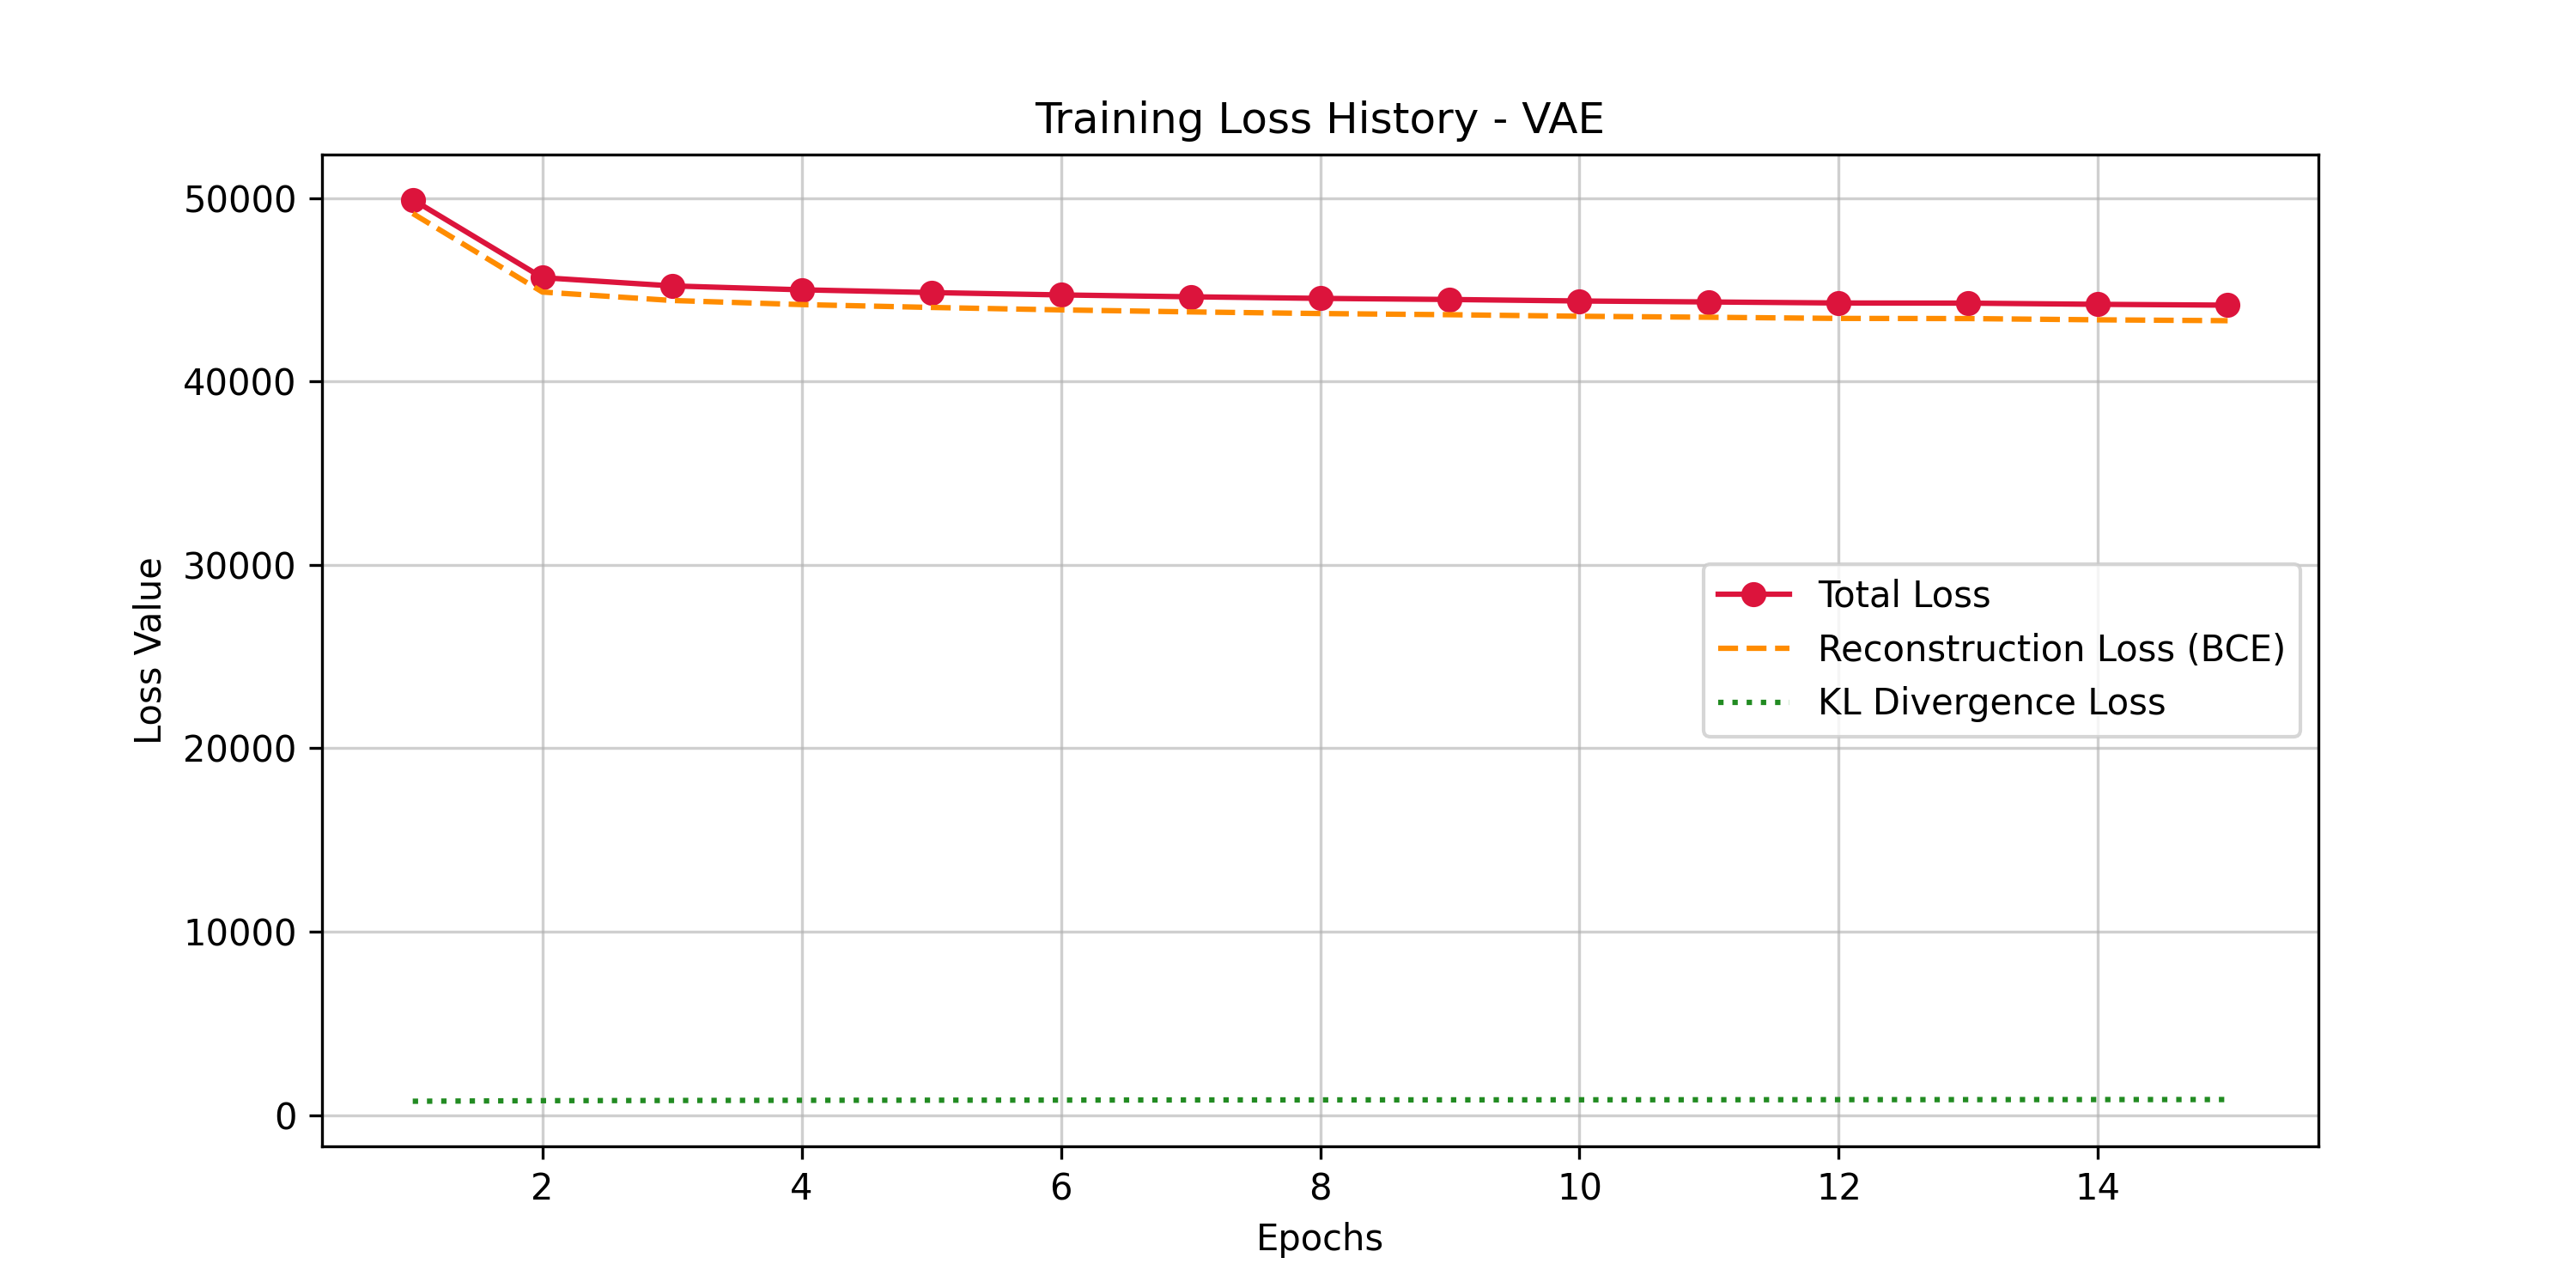
\includegraphics[width=0.8\textwidth]{../images/loss_history_dim2.png}
	\caption{Kurva Penurunan Nilai Training Loss pada Eksperimen VAE.}
	\label{fig:loss_graph}
\end{figure}

\section{Hasil Rekonstruksi Beberapa Ukuran Latent Dimension}
Sesuai dengan panduan eksperimen, pengujian dilakukan dengan membagi model ke dalam tiga variasi batasan dimensi ruang laten (\textit{bottleneck vector}): $2$, $8$, dan $32$. Dokumentasi visual dari hasil visualisasi uji coba perbandingan dapat dilihat di bawah ini.

\begin{figure}[htbp]
	\centering
	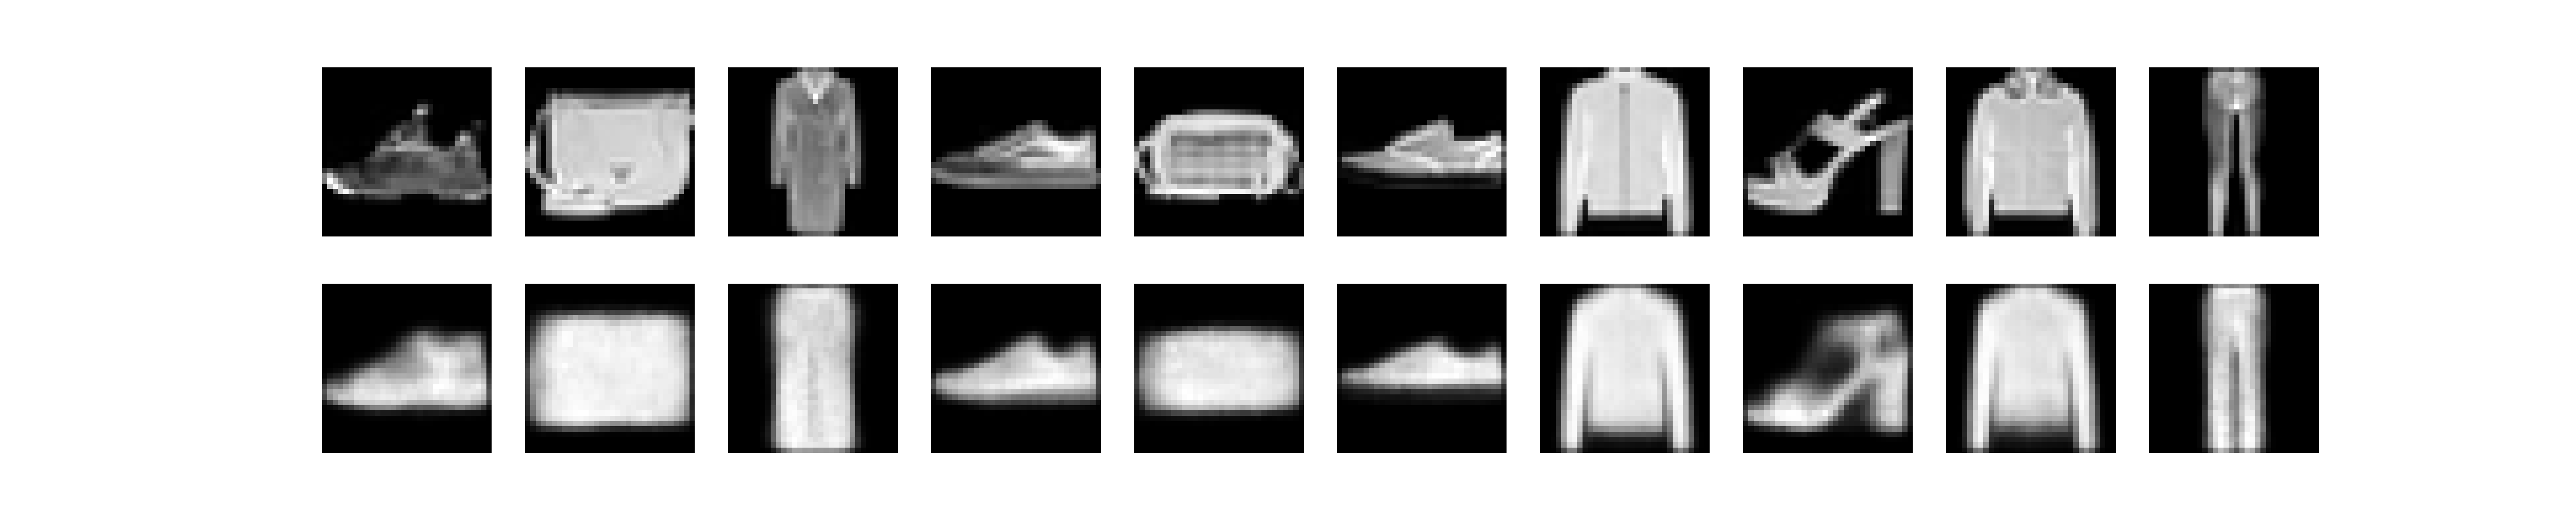
\includegraphics[width=0.9\textwidth]{../images/reconstruction_dim2.png}
	\caption{Hasil Rekonstruksi Citra pada Latent Dimension = 2.}
\end{figure}

\begin{figure}[htbp]
	\centering
	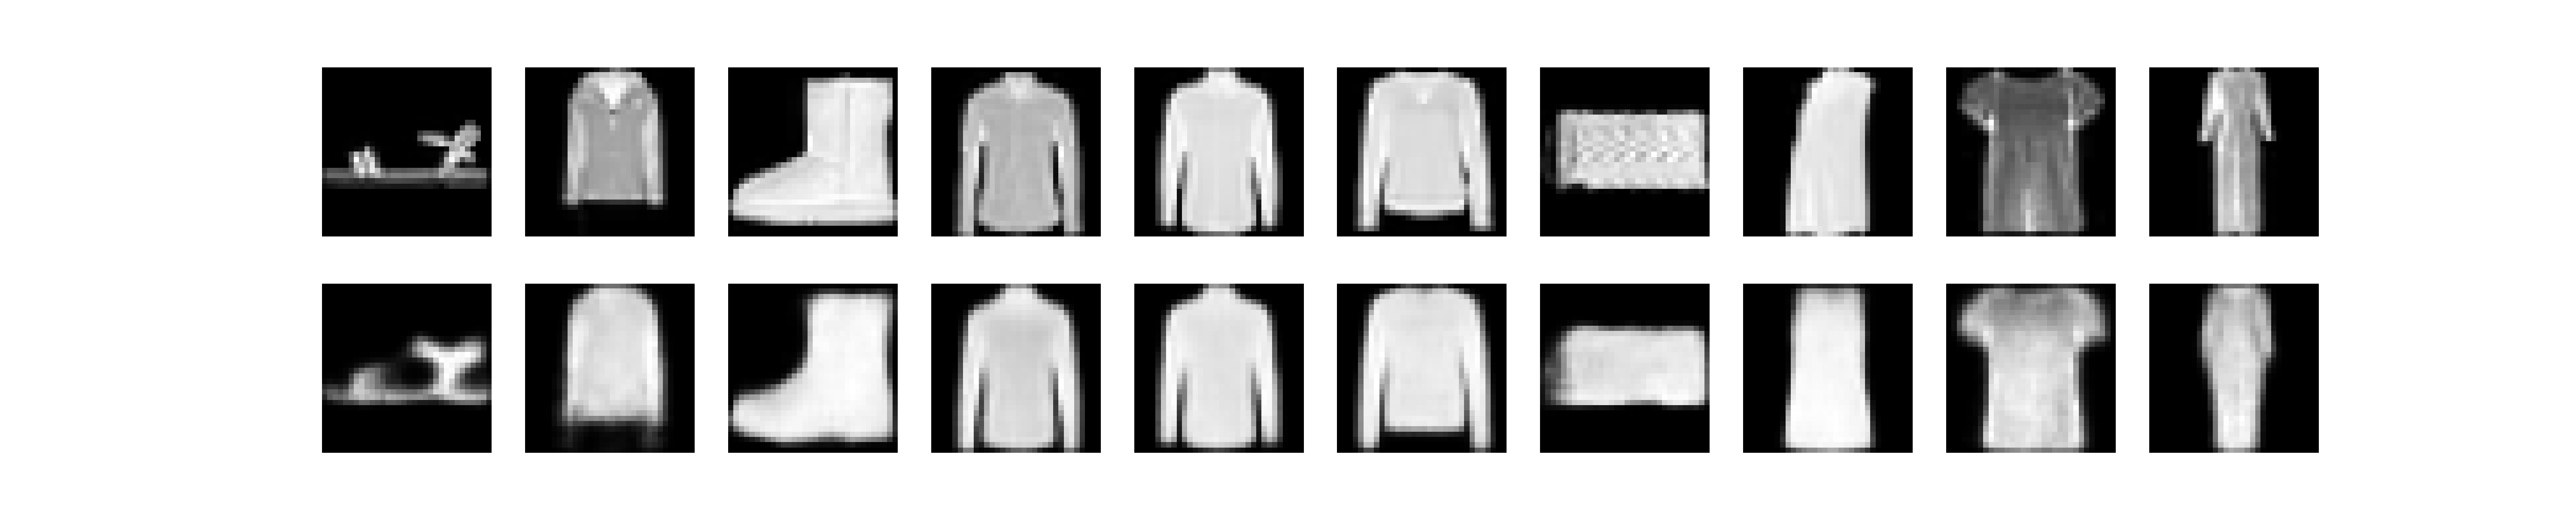
\includegraphics[width=0.9\textwidth]{../images/reconstruction_dim8.png}
	\caption{Hasil Rekonstruksi Citra pada Latent Dimension = 8.}
\end{figure}

\begin{figure}[htbp]
	\centering
	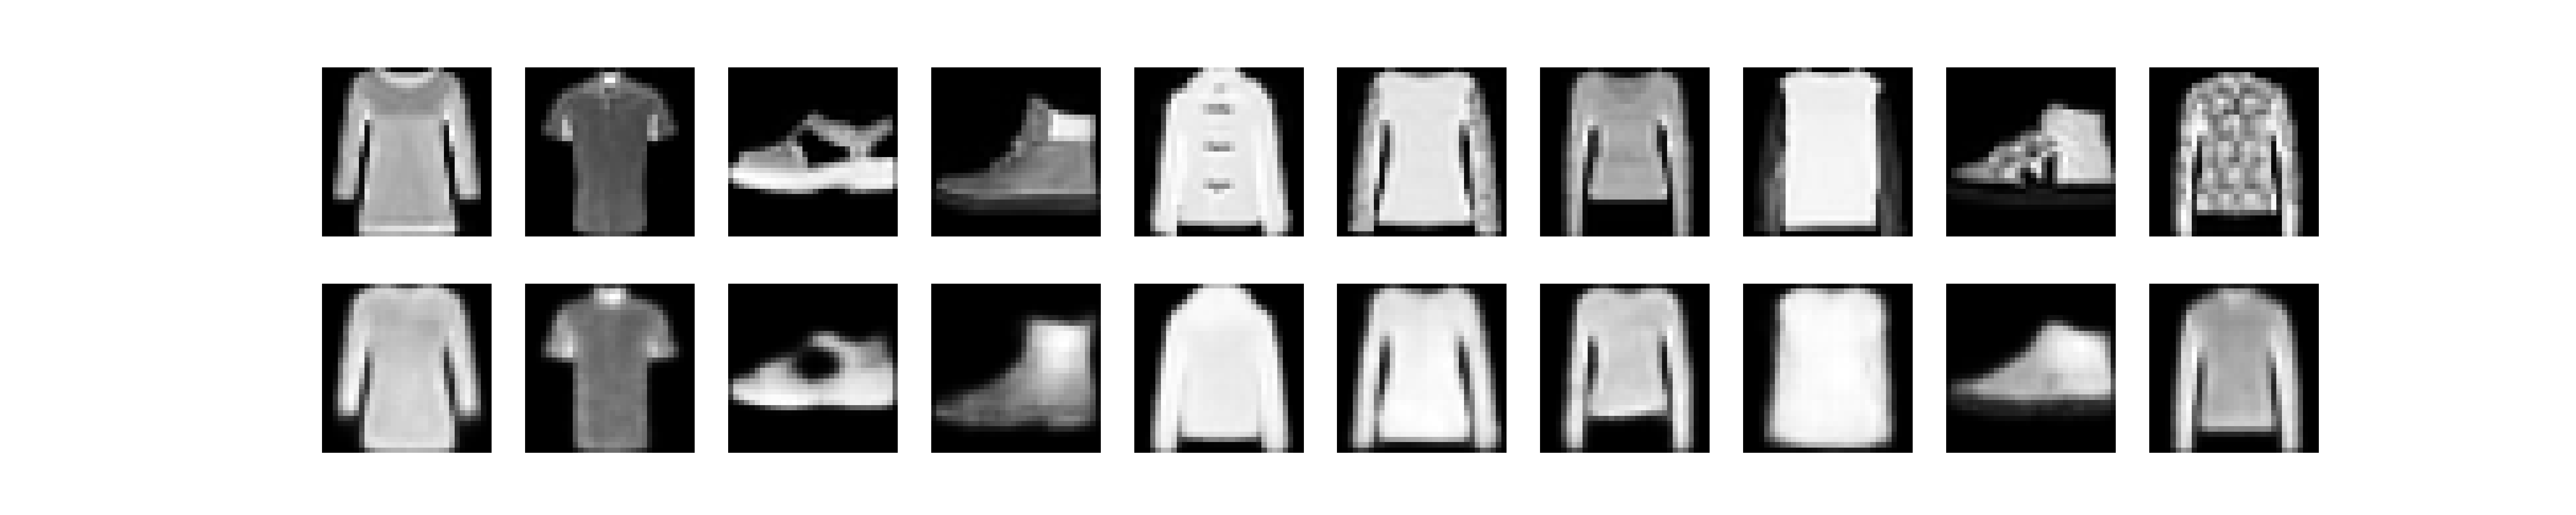
\includegraphics[width=0.9\textwidth]{../images/reconstruction_dim32.png}
	\caption{Hasil Rekonstruksi Citra pada Latent Dimension = 32.}
\end{figure}

\section{Penjelasan Cara Menjalankan Program dari Terminal}
Aplikasi program pemodelan ini telah di-refaktor penuh menjadi skrip mandiri Python (\textit{standalone scripts}) yang mendukung antarmuka CLI (\textbf{Command Line Interface}) berbasis pustaka bawaan \lstinline|argparse|.

\subsection{Proses Rekonstruksi Penuh (rekonstruksi.py)}
Skrip ini memuat arsitektur VAE secara utuh, mengambil citra asli dari dataset berdasarkan indeks, mengompresinya lewat encoder, lalu memproyeksikannya kembali lewat decoder untuk menghasilkan 3 luaran file gambar sekaligus (\lstinline|original.png|, \lstinline|reconstructed.png|, dan \lstinline|comparison.png|).

Perintah eksekusi di terminal:
\begin{lstlisting}[language=bash]
python reconstruct.py --model model_VAE_dim8.pth --index 25 --latent_dim 8
\end{lstlisting}


\section{Screenshot Terminal}
Berikut adalah bukti otentik pengujian running pengeksekusian program melalui sistem Command Prompt / Terminal lokal:

\begin{figure}[htbp]
	\centering
	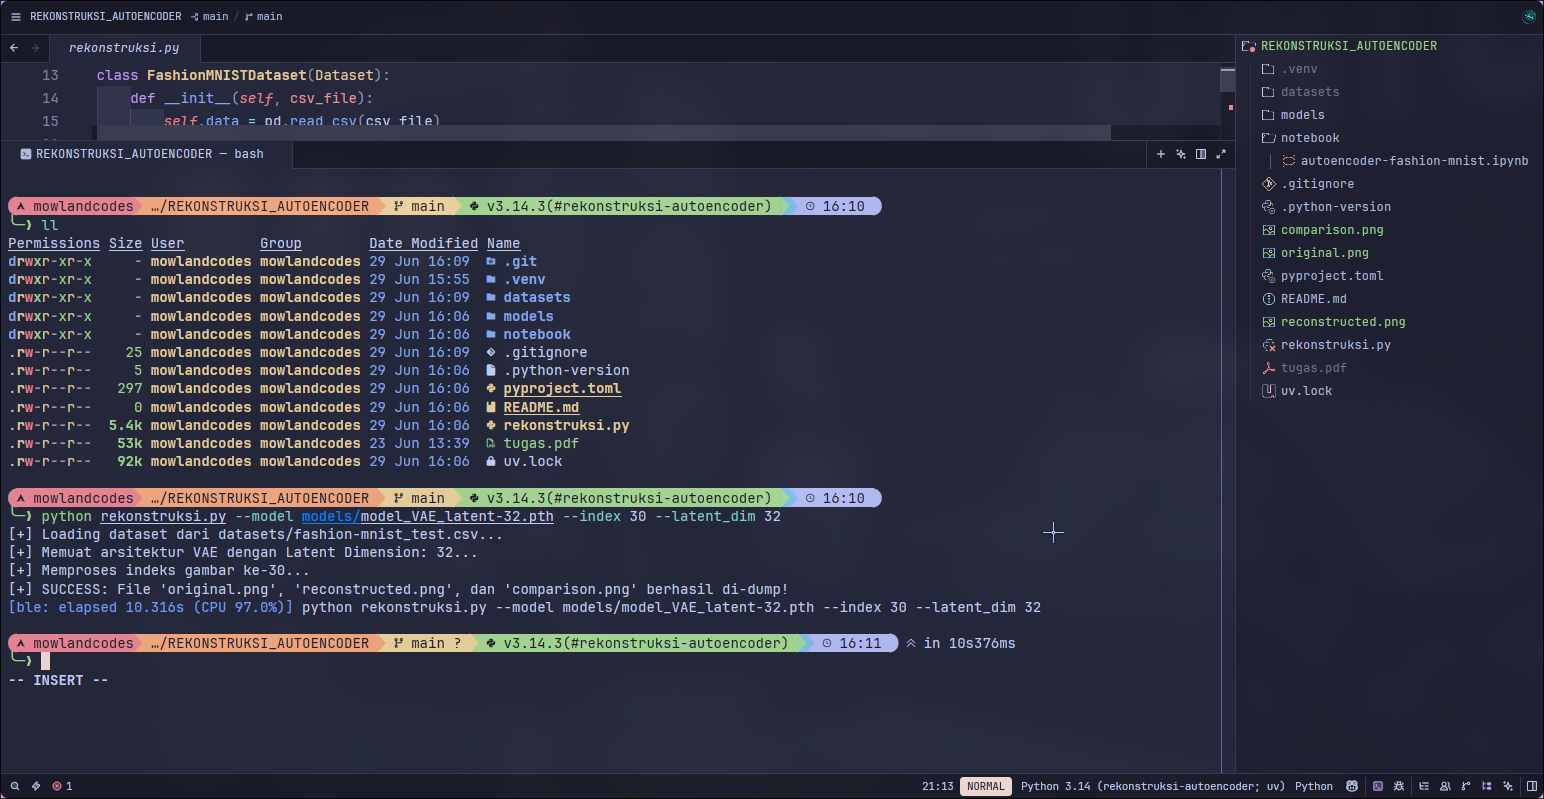
\includegraphics[width=0.8\textwidth]{../images/terminal_rekonstruksi.png}
	\caption{Dokumentasi Output Proses CLI Tools pada Command Line Interface.}
\end{figure}

\section{Analisis Hasil}
Bagian ini menyajikan analisis mendalam mengenai dinamika eksperimen Variational Autoencoder (VAE) pada dataset Fashion-MNIST. Seluruh temuan dari hasil pelatihan dan pengujian dievaluasi secara naratif untuk memahami korelasi fungsional antara komponen arsitektur jaringan dengan representasi visual yang dihasilkan.

\subsection{Mekanisme Kompresi Spasial dan Esensi Vektor Laten}
Proses rekonstruksi citra pada arsitektur VAE ini sangat bergantung pada pembagian kerja yang sinergis antara sub-jaringan \textbf{Encoder} dan \textbf{Decoder}. Dalam pipeline kompresi, \textbf{Encoder} berperan mengekstraksi fitur spasial esensial dari matriks piksel citra input berdimensi tinggi untuk direduksi ke dalam bentuk representasi laten berdimensi jauh lebih kecil. Melalui lapisan konvolusi, \textbf{Encoder} membuang redundansi informasi spasial kasar dan menyisakan intisari fitur manifold seperti pola umum, kontur pakaian, serta struktur geometris visual objek. Informasi padat ini disimpan dalam bentuk koordinat statistik kontinu berupa pasangan vektor rata-rata ($\mu$) dan log-varians ($\log \sigma^2$).

Penyimpanan data citra ke dalam bentuk \textbf{latent vector} ini menjadi sangat krusial karena bertindak sebagai ruang representasi fitur topologis abstrak, di mana model mengelompokkan karakteristik visual pakaian yang serupa ke dalam kedekatan jarak spasial. Lapisan \textbf{Decoder} mutlak membutuhkan konfigurasi \textbf{latent vector} ini sebagai acuan koordinat awal (\textbf{anchor point}). Tanpa adanya vektor referensi tersebut, lapisan dekonvolusi (\textit{ConvTranspose2d}) pada \textbf{Decoder} tidak akan memiliki basis orientasi matematis apa pun untuk melakukan operasi \textbf{up-sampling} guna membangun kembali representasi citra pakaian ke dimensi piksel aslinya.

\subsection{Implikasi Skalabilitas Kapasitas Laten Terhadap Fidelitas Visual}
Ukuran alokasi ruang pada \textbf{latent dimension} memegang kendali penuh terhadap tingkat keberhasilan proses rekonstruksi gambar. Berdasarkan hasil uji coba, ukuran \textbf{latent dimension} yang terlalu kecil, seperti pada dimensi 2, memicu terjadinya keterbatasan kapasitas penampungan data (\textbf{information bottleneck constraint}). Karena dipaksa memeras fitur gambar pakaian serumit dataset Fashion-MNIST hanya ke dalam dua variabel numerik, sebagian besar detail mikro dari citra input terpaksa dieliminasi oleh model. Dampak visual yang dihasilkan adalah citra rekonstruksi tampak jauh lebih buram (\textbf{blurry}), kehilangan tekstur tajam, dan hanya mampu menampilkan siluet besar dari luar objek.

Sebaliknya, ketika ukuran \textbf{latent dimension} diperluas menjadi dimensi 8 dan mencapai performa puncaknya pada dimensi 32, kualitas visual hasil rekonstruksi mengalami peningkatan kualitas yang masif. Kapasitas ruang penampungan informasi yang lebih luas meminimalkan efek kerusakan data akibat kompresi (\textbf{lossy compression effect}), sehingga memberikan fleksibilitas tinggi bagi lapisan \textbf{Decoder} untuk menyusun kembali detail-detail rumit pakaian secara presisi. Hubungan komparatif fungsional antara kapasitas ruang laten, nilai evaluasi akhir, serta impresi visual hasil pengujian dirangkum secara ringkas pada Tabel~\ref{tab:perbandingan_latent}.

\begin{table}[htbp]
	\centering
	\caption{Tabel Komparasi Performa dan Kualitas Visual}
	\label{tab:perbandingan_latent}
	\resizebox{1.0\textwidth}{!}{
		\begin{tabular}{@{}cccc@{}}
			\toprule
			\textbf{Ukuran Latent} & \textbf{Final Loss Value} & \textbf{Ketajaman Visual} & \textbf{Kehilangan Detail}      \\ \midrule
			Dimension = 2          & $\approx 44163.6697$      & Sangat Buram / Abstrak    & Tinggi (Hanya Siluet)           \\
			Dimension = 8          & $\approx 41052.3780$      & Cukup Jelas / Bertekstur  & Sedang (Detail Mikro Hilang)    \\
			Dimension = 32         & $\approx 40976.0432$      & Lumayan Tajam / Identik   & Rendah (Presisi Lumayan Tinggi) \\ \bottomrule
		\end{tabular}
	}
\end{table}

Pengamatan terhadap dinamika kurva pelatihan juga menunjukkan adanya korelasi linear yang kuat antara nilai akumulasi \textbf{loss} dengan kualitas visual hasil rekonstruksi. Semakin kecil nilai akhir fungsional \textit{Binary Cross Entropy} (BCE) yang dicapai oleh model (dari nilai $\approx 44163.6697$ pada dimensi 2 hingga menyusut ke angka $\approx 40976.0432$ pada dimensi 32), maka semakin identik pula distribusi proyeksi nilai piksel buatan \textbf{Decoder} terhadap nilai piksel dari citra target asli. Penurunan nilai \textbf{loss} secara konsisten menjadi indikator valid bahwa \textbf{weights} dari model sedang mengalami konvergensi optimal untuk memperkecil distorsi visual gambar sintetis.

\subsection{Evaluasi Teknis Inferensi Terminal dan Kapabilitas Generatif Model}
Sesuai dengan standarisasi ketentuan teknis tugas, proses pelatihan diisolasi pada platform Kaggle Notebook, sedangkan proses inferensi dijalankan melalui arsitektur terpisah via Command Line Interface (CLI) terminal lokal. Secara matematis, tidak ada perbedaan fungsional pada hasil rekonstruksi citra yang dijalankan di notebook maupun terminal, karena kedua lingkungan tersebut memuat berkas bobot parameter (\textbf{weights} file \lstinline|.pth|) yang identik. Namun, eksekusi melalui terminal menuntut jaminan kesesuaian arsitektur model yang sangat ketat antara fase pelatihan (\textit{training}) dan fase inferensi. Ketidaksesuaian kecil pada deklarasi jumlah \textit{layer} linear atau dimensi variabel laten pada skrip terminal akan memicu kegagalan sistem secara fatal (\textbf{runtime size mismatch error}) karena ketidakselarasan ukuran matriks bobot memori komputer.

Kemampuan generatif sejati dari arsitektur ini teruji ketika skrip generator dipicu dengan menyuntikkan nilai \textbf{latent vector} secara acak (\textbf{random continuous sampling}). Kualitas citra pakaian yang diproduksi oleh lapisan \textbf{Decoder} ternyata tetap terjaga bentuk geometrisnya dengan baik dan tidak hancur menjadi sekadar kumpulan \textbf{noise} acak biasa. Fenomena ini membuktikan sifat kontinuitas manifold ruang laten yang dikontrol ketat oleh regulasi komponen \textbf{KL Divergence}.

Aspek terakhir ini membuktikan bahwasanya model Variational Autoencoder ini \textbf{bener-bener memahami struktur geometris gambar} pakaian secara mendalam, bukan sekadar belajar menyalin kaku (\textbf{memorizing/copying}) susunan posisi piksel input. Melalui kombinasi fungsional loss, model berhasil mengasimilasi aturan semantik semesta data, seperti memahami konsep simetrisitas bentuk lengan baju, orientasi kerah, hingga lengkungan sol sepatu. Kemampuan melakukan interpolasi mulus dan melahirkan variasi gambar baru dari koordinat laten acak menjadi bukti otentik keberhasilan generalisasi fitur terstruktur pada proyek tugas besar ini.

\section{Kesimpulan}
Eksperimen pembuktian ini menunjukkan bahwasanya ukuran penentuan \textit{latent dimension} memegang peranan krusial sebagai \textit{information bottleneck} di dalam pemodelan arsitektur Autoencoder dan VAE. Semakin besar ukuran dimensi ruang laten yang dialokasikan, maka tingkat keakuratan hasil rekonstruksi citra akan berbanding lurus menjadi semakin tinggi karena hilangnya data (\textit{loss of information}) akibat kompresi dapat diminimalisir. Penggunaan metode regulasi probabilitas kontinu VAE juga terbukti tangguh untuk mengonstruksi ruang laten terstruktur yang berpotensi penuh sebagai pilar utama pemodelan generatif sintetis.

\end{document}
